%%%%%%%%%%%%%%%%%%%%%%%%%%%%%%%%%%%%%%%%%%%%%%%%%%%%%%%%%%%%%%%%%%%%%%%%
%                                                                      %
%     File: Implementation/01_SimulationEnvironment.tex                %
%     Tex Master: ../Thesis.tex                                        %
%                                                                      %
%%%%%%%%%%%%%%%%%%%%%%%%%%%%%%%%%%%%%%%%%%%%%%%%%%%%%%%%%%%%%%%%%%%%%%%%

% ==============================================================================
\section{Simulation Environment}
\label{sec:simulation_environment}

Simulation is the natural first step in the development of the controllers, since it allows them to be tested and adjusted before being used on the real vehicles. The simulations in this work are run in Gazebo \cite{koenig2004gazebo}, a robotics simulator. A simulator is a program that creates a virtual environment, places robots in it, and calculates how they would behave in reality. At each step, it receives the commands sent to the robots, computes the forces acting on them, updates their positions accordingly, and returns the measurements that their sensors would produce. To the controller, the simulated robot behaves like a real one.

This allows controllers to be developed through many fast iterations, and different scenarios to be repeated under the same conditions, which makes the comparison between controllers and parameter choices fair. Sensor noise and estimation error can also be included in simulation, but they can be left out during development, so that the behaviour of the controllers is first analysed on its own.

\subsection{World}
\label{sec:world}

The space where the simulation takes place is called the world. It contains the environment around the robots, such as the terrain, obstacles, and light, and defines the rules that apply inside it, such as the way time advances, the physical effects that are calculated, and the sensors that can be simulated. The robots are not part of the world. They are added to it afterwards, and what happens to them results from the interaction between their own models and the world in which they are placed.

A world is defined in a text file that lists its elements and the plugins that enable its behaviour. Plugins are software modules that add functionality to the simulator, such as the calculation of buoyancy or the simulation of sensors.

The world used in this work represents an open water area, shown in Figure~\ref{fig:world_view}. It consists of a sea surface and a seabed below it, and the buoyancy is calculated from the density of the water, which allows the hull of the \gls{usv} to float. The world also enables the simulation of the sensors that the vehicles can use to estimate their state, such as inertial, magnetic, pressure, and satellite positioning sensors.

\begin{figure}[!htbp]
    \centering
    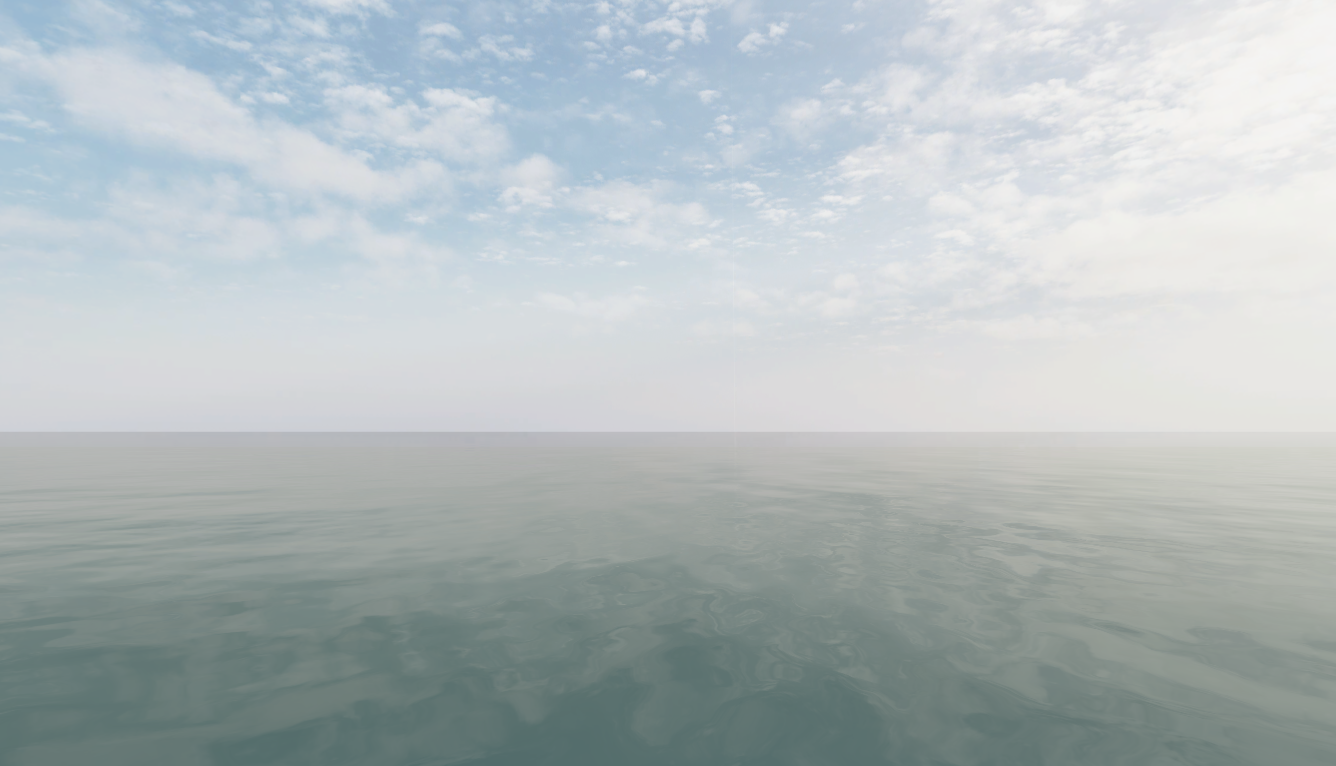
\includegraphics[width=0.7\textwidth]{Implementation/figures/01_simulation_environment/world.png}
    \caption{View of the simulated world.}
    \label{fig:world_view}
\end{figure}

The vehicles operate at sea, where wind, waves, and currents act on them. The world allows these disturbances to be included, so that the controllers can be tested under conditions that their models do not predict. Each disturbance acts through a different physical path. Wind applies a force on the bodies exposed to the air, waves change the height of the water surface and therefore the buoyancy of the hull, and currents move the water itself, which changes the drag on the submerged bodies. These disturbances can be enabled, disabled, or adjusted for each test. In this work, a moderate sea, with a significant wave height of $0.6\,\text{m}$, is present in every test unless stated otherwise.


%%%%%%%%%%%%%%%%%%%%%%%%%%%%%%%%%%%%%%%%%%%%%%%%%%%%%%%%%%%%%%%%%%%%%%%%
\subsection{Wave Adaptive Modular Vessel}
\label{sec:usv_model}

The \gls{wamv} is a catamaran with two inflatable hulls connected by a central payload deck, used in maritime robotics competitions. In this work it is the \gls{usv} of the tethered system. It was chosen mainly because its payload deck is large enough to serve as a platform for the takeoff and landing of the \gls{uav}. In addition, a complete and publicly available model of the \gls{usv} exists in the \gls{vrx} simulation framework \cite{bingham2019vrx}, so that the work could focus on the control and not on building and validating a \gls{usv} model. Figure~\ref{fig:wamv_render} shows the vehicle in the simulated world.

\begin{figure}[!htbp]
    \centering
    \includegraphics[width=0.7\textwidth]{Implementation/figures/01_simulation_environment/wamv.png}
    \caption{The \gls{wamv} catamaran in the simulated world.}
    \label{fig:wamv_render}
\end{figure}

In the simulator, a vehicle is described by a model that lists its bodies, the joints that connect them, and for each body its mass, its inertia, and its geometry. The \gls{wamv} is represented by a main rigid body, which includes the hulls, the deck, the batteries, and the mass of the thrusters, propellers, and sensors, with a total mass of $259.10\,\text{kg}$ and moments of inertia of $219$, $568$, and $683\,\text{kg}\cdot\text{m}^2$ about the longitudinal, lateral, and vertical axes. The thrusters, propellers, and sensors are also modelled as separate bodies attached to it through joints, with negligible mass. The thrusters can rotate to steer the \gls{usv}, while the joints of the sensors are fixed. As the thrusters are mounted far aft, the centre of gravity of the whole vehicle lies $0.29\,\text{m}$ behind the centre of the hull geometry. The origin and the centre of mass of the main body are placed at this point, which is where the hydrodynamic forces described next are applied and which the odometry of the simulator refers to.

The catamaran has an overall length of $4.90\,\text{m}$ and a beam of $2.40\,\text{m}$. The payload deck, with $1.85\,\text{m}$ in length and $1.00\,\text{m}$ in width, is supported by the two hulls at about $1.25\,\text{m}$ above the water surface, as shown in Figure~\ref{fig:wamv_schematic}.

\begin{figure}[htbp]
    \centering
    \subfloat[Top view.]{
        \begin{tikzpicture}[
            dimension/.style={draw, <->, >={Stealth[length=4pt]}, thin, dashed, gray},
            pointer/.style={draw, ->, >={Stealth[length=4pt]}, thin, gray}
        ]
            \node[anchor=south west, inner sep=0] (image) at (0,0) {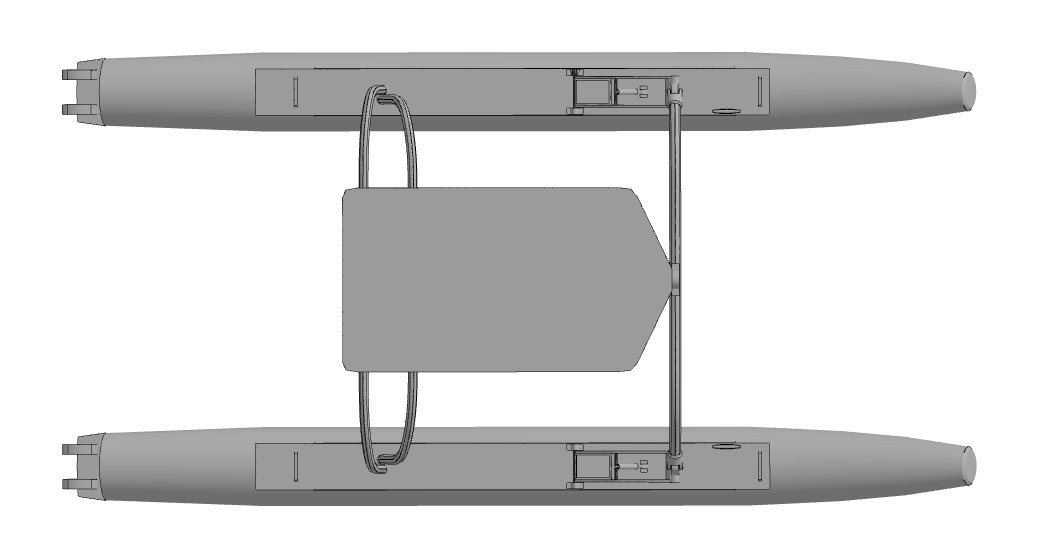
\includegraphics[width=0.40\textwidth]{Implementation/figures/01_simulation_environment/wamv_top_view.png}};
            \begin{scope}[x={(image.south east)},y={(image.north west)}]
                % Overall Length (4.90m)
                \draw[gray, thin] (0.06, 0.88) -- (0.06, 0.96);
                \draw[gray, thin] (0.94, 0.88) -- (0.94, 0.96);
                \draw[dimension] (0.06, 0.93) -- (0.94, 0.93);
                \node at (0.50, 0.96) [font=\scriptsize, above] {$4.90\,\text{m}$};

                % Overall Beam (2.40m nominal)
                \draw[gray, thin] (0.02, 0.07) -- (0.07, 0.07);
                \draw[gray, thin] (0.02, 0.92) -- (0.07, 0.92);
                \draw[dimension] (0.05, 0.07) -- (0.05, 0.92);
                \node at (0.05, 0.5) [font=\scriptsize, rotate=90, above] {$2.40\,\text{m}$};

                % Component Labels
                \node (hull_lbl) at (0.20, 0.50) [font=\scriptsize, draw, rounded corners=1pt, fill=white, inner sep=2pt] {Hulls};
                \draw[pointer] (hull_lbl.north) -- (0.30, 0.84);
                \draw[pointer] (hull_lbl.south) -- (0.30, 0.16);

                \node (deck_lbl) at (0.80, 0.35) [font=\scriptsize, draw, rounded corners=1pt, fill=white, inner sep=2pt] {Payload Deck};
                \draw[pointer] (deck_lbl.west) -- (0.55, 0.50);

                % Payload Deck Length (1.85m)
                \draw[gray, thin] (0.334, 0.3) -- (0.334, 0.23);
                \draw[gray, thin] (0.65, 0.3) -- (0.65, 0.23);
                \draw[dimension] (0.334, 0.27) -- (0.65, 0.27);
                \node at (0.50, 0.27) [font=\scriptsize, fill=white, inner sep=1pt] {$1.85\,\text{m}$};

                % Payload Deck Width (1.00m)
                \draw[gray, thin] (0.334, 0.315) -- (0.29, 0.315);
                \draw[gray, thin] (0.334, 0.65) -- (0.29, 0.65);
                \draw[dimension] (0.31, 0.315) -- (0.31, 0.65);
                \node at (0.31, 0.495) [font=\scriptsize, rotate=90, fill=white, inner sep=1pt] {$1.00\,\text{m}$};
            \end{scope}
        \end{tikzpicture}
        \label{fig:wamv_top}
    }
    \hfill
    \subfloat[Side view.]{
        \begin{tikzpicture}[
            dimension/.style={draw, <->, >={Stealth[length=4pt]}, thin, dashed, gray}
        ]
            \node[anchor=south west, inner sep=0] (image) at (0,0) {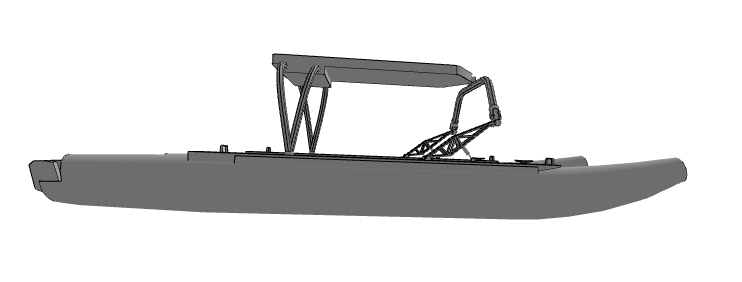
\includegraphics[width=0.40\textwidth]{Implementation/figures/01_simulation_environment/wamv_side_view.png}};
            \begin{scope}[x={(image.south east)},y={(image.north west)}]
                % Water Level
                \draw[gray, thick, dashed] (0.02, 0.28) -- (0.92, 0.28) node[right, font=\scriptsize] {Water Level};

                % Deck Height (1.25m above water level)
                \draw[gray, thin] (0.64, 0.77) -- (0.75, 0.77);
                \draw[gray, thin] (0.68, 0.28) -- (0.75, 0.28);
                \draw[dimension] (0.72, 0.28) -- (0.72, 0.77);
                \node at (0.72, 0.525) [font=\scriptsize, right] {$1.25\,\text{m}$};
            \end{scope}
        \end{tikzpicture}
        \label{fig:wamv_side}
    }
    \caption{WAM-V catamaran layout.}
    \label{fig:wamv_schematic}
\end{figure}

The behaviour of the \gls{usv} on the water is determined by how the simulator reproduces the forces that the water exerts on it. The hulls are kept afloat by a buoyancy force, which is calculated from the volume of each hull below the water surface. When waves are present, this volume changes along the hulls and the catamaran pitches and rolls accordingly. As the \gls{usv} moves, the water also resists its motion through drag forces and moments applied in the six degrees of freedom. For a velocity $\nu_i$ along or about each degree of freedom, the drag is
\begin{equation}
    D_i = -\left(d_i^{\text{lin}} + d_i^{\text{quad}}\,|\nu_i|\right)\nu_i,
    \label{eq:usv_drag}
\end{equation}
where $d_i^{\text{lin}}$ and $d_i^{\text{quad}}$ are the linear and quadratic coefficients. The negative sign makes the drag oppose the motion, and the linear term dominates at low speeds while the quadratic term dominates at higher speeds. This makes the vehicle slow down naturally when the propulsion is cut off. The coefficients of each degree of freedom, given in Table~\ref{tab:usv_damping_parameters}, are those provided by the \gls{vrx} model.

\begin{table}[htbp]
    \centering
    \caption{Hydrodynamic damping coefficients of the simulated \gls{wamv}.}
    \label{tab:usv_damping_parameters}
    \begin{tabular}{lccc}
        \toprule
        \textbf{Damping Mode} & \textbf{Linear Coefficient} & \textbf{Quadratic Coefficient} & \textbf{Unit} \\
        \midrule
        Surge & $100.00$ & $150.00$ & $\text{N}/(\text{m/s})$ or $\text{N}/(\text{m/s})^2$ \\
        Sway & $100.00$ & $100.00$ & $\text{N}/(\text{m/s})$ or $\text{N}/(\text{m/s})^2$ \\
        Heave & $500.00$ & -- & $\text{N}/(\text{m/s})$ \\
        Roll & $300.00$ & $600.00$ & $\text{N}\cdot\text{m}/(\text{rad/s})$ or $\text{N}\cdot\text{m}/(\text{rad/s})^2$ \\
        Pitch & $900.00$ & $900.00$ & $\text{N}\cdot\text{m}/(\text{rad/s})$ or $\text{N}\cdot\text{m}/(\text{rad/s})^2$ \\
        Yaw & $800.00$ & $800.00$ & $\text{N}\cdot\text{m}/(\text{rad/s})$ or $\text{N}\cdot\text{m}/(\text{rad/s})^2$ \\
        \bottomrule
    \end{tabular}
\end{table}

The vehicle is propelled by two azimuth thrusters, one at the stern of each hull, and it steers by rotating them instead of using a rudder. To move, the model needs to receive, for each thruster, the thrust force that it must produce, in newtons, and its steering angle. The angle is limited to $\pm 30$ degrees, to avoid twisting the power cables, and its rate of change to $10$ degrees per second. The thrust is limited to $510.0\,\text{N}$ in the forward direction, a value representative of the electric outboard motors used on the \gls{wamv} in robotics competitions, such as the Torqeedo Cruise 2.0 \cite{torqeedo_cruise_manual}. In reverse, the propeller is less efficient, which is modelled with a multiplier of $0.746$ that limits the thrust to $-380.0\,\text{N}$.

%%%%%%%%%%%%%%%%%%%%%%%%%%%%%%%%%%%%%%%%%%%%%%%%%%%%%%%%%%%%%%%%%%%%%%%%
\subsection{\texorpdfstring{x500 \Gls{uav}}{x500 UAV}}
\label{sec:x500_quadrotor}

The Holybro X500 v2 \cite{holybro_x500} is a \gls{uav}, and in this work it is the aerial vehicle of the tethered system. It was chosen mainly because it is heavier and more stable than small \glspl{uav}, which makes it better suited to fly with a tether attached to it. Its size is also compatible with the payload deck of the \gls{wamv}, leaving enough room for takeoff and landing, and a complete model of the vehicle is available in the simulation ecosystem of the PX4 autopilot \cite{meier2015px4}, so that the work could focus on the control and not on building and validating a vehicle model. Figure~\ref{fig:x500_render} shows the vehicle in the simulated world.

\begin{figure}[!htbp]
    \centering
    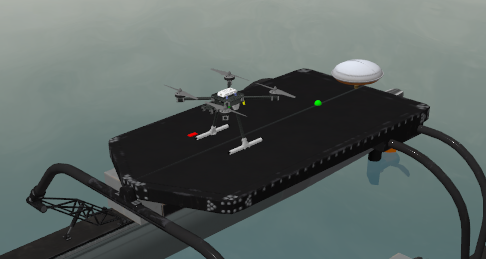
\includegraphics[width=0.7\textwidth]{Implementation/figures/01_simulation_environment/drone_world.png}
    \caption{The x500 \gls{uav} in the simulated world.}
    \label{fig:x500_render}
\end{figure}

The x500 is described in the simulator in the same way as the \gls{wamv}, by a model that lists its bodies, the joints that connect them, and the mass and inertia of each one. It consists of a main rigid body, which includes the frame and the sensors, and of four rotors, which are separate bodies connected to it through rotating joints. Their masses, inertias, and positions are given in Table~\ref{tab:x500_parameters}. The rotors are $0.348\,\text{m}$ apart along the sides of the frame and about $0.49\,\text{m}$ apart along the diagonal. The landing gear is $0.264\,\text{m}$ wide, and the motor mounts are $0.26\,\text{m}$ above the ground, as shown in Figure~\ref{fig:x500_schematic}.

\begin{figure}[!htbp]
    \centering
    \subfloat[Top view.]{
        \begin{tikzpicture}[
            dimension/.style={draw, <->, >=stealth, thin, dashed, gray},
            ext/.style={draw, gray, thin},
            center/.style={fill=gray, draw=none, circle, inner sep=0.8pt}
        ]
            \node[anchor=south west, inner sep=0] (image) at (0,0) {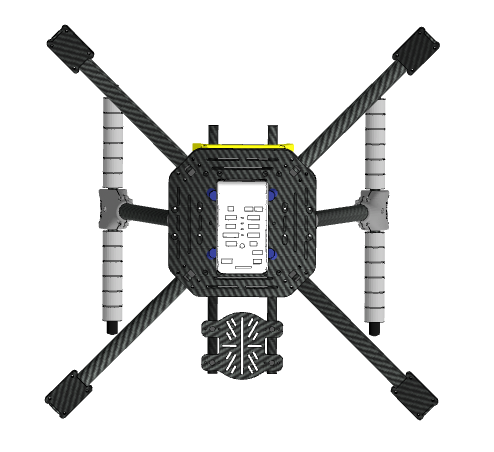
\includegraphics[width=0.34\textwidth]{Implementation/figures/01_simulation_environment/drone_top_view.png}};
            \begin{scope}[x={(image.south east)},y={(image.north west)}]
                % Rotor centres (TL, TR, BL, BR)
                \coordinate (TL) at (0.142, 0.894);
                \coordinate (TR) at (0.844, 0.894);
                \coordinate (BL) at (0.142, 0.122);
                \coordinate (BR) at (0.844, 0.122);
                \node[center] at (TL) {};
                \node[center] at (TR) {};
                \node[center] at (BL) {};
                \node[center] at (BR) {};

                % Rotor spacing along the frame sides (0.348 m), horizontal
                \draw[ext] (0.142, 0.945) -- (0.142, 0.985);
                \draw[ext] (0.844, 0.945) -- (0.844, 0.985);
                \draw[dimension] (0.142, 0.968) -- (0.844, 0.968);
                \node[font=\tiny, fill=white, inner sep=1pt] at (0.493, 0.968) {$0.348\,\text{m}$};

                % Rotor spacing along the frame sides (0.348 m), vertical
                \draw[ext] (0.088, 0.894) -- (0.022, 0.894);
                \draw[ext] (0.088, 0.122) -- (0.022, 0.122);
                \draw[dimension] (0.035, 0.894) -- (0.035, 0.122);
                \node[font=\tiny, rotate=90, fill=white, inner sep=1pt] at (0.035, 0.508) {$0.348\,\text{m}$};

                % Rotor spacing along the diagonal (0.49 m)
                \draw[<->, >=stealth, thin, dashed, white] (TL) -- (BR);
                \node[font=\tiny, rotate=-45, fill=white, inner sep=1pt] at ($(TL)!0.19!(BR)$) {$0.49\,\text{m}$};
            \end{scope}
        \end{tikzpicture}
        \label{fig:x500_top}
    }
    \hfill
    \subfloat[Front view.]{
        \begin{tikzpicture}[
            dimension/.style={draw, <->, >=stealth, thin, dashed, gray},
            ext/.style={draw, gray, thin},
            center/.style={fill=gray, draw=none, circle, inner sep=0.8pt}
        ]
            \node[anchor=south west, inner sep=0] (image) at (0,0) {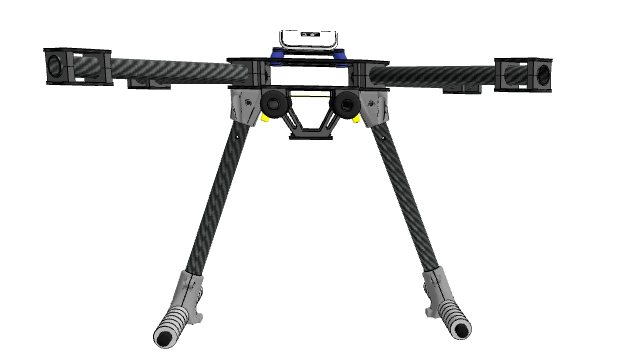
\includegraphics[width=0.52\textwidth]{Implementation/figures/01_simulation_environment/drone_side_view.png}};
            \begin{scope}[x={(image.south east)},y={(image.north west)}]
                % Reference points: centre of the left motor mount and centres of the two feet
                \node[center] at (0.123, 0.814) {};
                \node[center] at (0.259, 0.061) {};
                \node[center] at (0.734, 0.086) {};

                % Height: from the ground (bottom of the feet) to the motor mounts (0.26 m)
                \draw[ext] (0.062, 0.814) -- (0.012, 0.814);
                \draw[ext] (0.235, 0.040) -- (0.012, 0.040);
                \draw[dimension] (0.025, 0.040) -- (0.025, 0.814);
                \node[font=\tiny, rotate=90, fill=white, inner sep=1pt] at (0.025, 0.427) {$0.26\,\text{m}$};

                % Base width: between the centres of the feet (0.264 m)
                \draw[ext] (0.259, 0.035) -- (0.259, -0.120);
                \draw[ext] (0.734, 0.060) -- (0.734, -0.120);
                \draw[dimension] (0.259, -0.100) -- (0.734, -0.100);
                \node[font=\tiny, fill=white, inner sep=1pt] at (0.4965, -0.100) {$0.264\,\text{m}$};
            \end{scope}
        \end{tikzpicture}
        \label{fig:x500_front}
    }
    \caption{x500 \gls{uav} layout.}
    \label{fig:x500_schematic}
\end{figure}

\begin{table}[!htbp]
    \centering
    \caption{Parameters of the simulated x500, based on the PX4 model \cite{px4_x500_model}.}
    \label{tab:x500_parameters}
    \begin{tabular}{lcc}
        \toprule
        \textbf{Parameter} & \textbf{Value} & \textbf{Unit} \\
        \midrule
        Main body mass & $2.0$ & $\text{kg}$ \\
        Rotor mass (each) & $0.016$ & $\text{kg}$ \\
        Total mass & $2.06$ & $\text{kg}$ \\
        Moment of inertia, longitudinal and lateral axes & $0.0217$ & $\text{kg}\cdot\text{m}^2$ \\
        Moment of inertia, vertical axis & $0.040$ & $\text{kg}\cdot\text{m}^2$ \\
        Rotor position, along each horizontal axis & $\pm 0.174$ & $\text{m}$ \\
        \midrule
        Thrust coefficient $k_F$ & $1.11\times 10^{-5}$ & $\text{N}/(\text{rad/s})^2$ \\
        Moment coefficient $k_M$ & $0.016$ & $\text{m}$ \\
        Rotor drag coefficient $c_{drag}$ & $8.06\times 10^{-5}$ & $\text{N}\cdot\text{s}/\text{rad}\cdot\text{m}$ \\
        Minimum rotor speed & $150$ & $\text{rad/s}$ \\
        Maximum rotor speed & $1000$ & $\text{rad/s}$ \\
        Rotor time constant, accelerating & $12.5$ & $\text{ms}$ \\
        Rotor time constant, decelerating & $25$ & $\text{ms}$ \\
        \bottomrule
    \end{tabular}
\end{table}

The vehicle is lifted by the thrust that its rotors produce by pushing air downwards. The model receives, for each rotor $i$, a command with its angular speed $\omega_i$, in rad/s, and each rotor produces a thrust force $F_i$ and a reaction moment $M_i$ that depend on it \cite{mahony2012multirotor},
\begin{equation}
    F_i = k_F\,\omega_i^2, \qquad M_i = s_i\,k_M\,F_i,
    \label{eq:x500_rotor}
\end{equation}
where $k_F$ is the thrust coefficient, $k_M$ is the moment coefficient, and $s_i = \pm 1$ gives the sign of the moment, which depends on the direction of rotation. Rotors on the same diagonal rotate in the same direction and adjacent rotors in opposite directions, so that the reaction moments balance each other when the vehicle hovers. The model also includes the aerodynamic drag of the rotors.

The rotors have limits that the model reproduces. The speed of each rotor does not change instantly, and it follows the command with the time constants given in Table~\ref{tab:x500_parameters}, up to the maximum speed given in the same table. At this speed, each rotor produces about $11.1\,\text{N}$, and the four together produce $44.5\,\text{N}$. As the weight of the vehicle is $20.2\,\text{N}$, the thrust-to-weight ratio is about $2.2$. In hovering, the rotors produce about $45\%$ of their maximum thrust, at a speed of about $675\,\text{rad/s}$, which leaves about $24\,\text{N}$ available to manoeuvre and to counter the force of the tether.

%%%%%%%%%%%%%%%%%%%%%%%%%%%%%%%%%%%%%%%%%%%%%%%%%%%%%%%%%%%%%%%%%%%%%%%%
\subsection{Tether}
\label{sec:tether}

The tether couples the two vehicles, so the behaviour of the system depends on how it is represented. To evaluate the controllers as close as possible to real operation, they should be tested against a tether model that is more detailed than the one used in their design. The model used by the controllers, described in Section~\ref{sec:system_modeling}, approximates the tether by a catenary linearised around a constant slack. This simplification keeps the computational cost low, since the controllers evaluate the model at every step of the prediction horizon within each sampling interval. The simulated tether does not have this constraint, so a more detailed model can be used. Since this type of tether is not included in the vehicle models, it is simulated separately and coupled to them.

The tether is simulated with MoorDyn \cite{hall2015moordyn}, a tool that represents a tether as a chain of lumped masses connected by segments that behave as springs and dampers. Each segment resists stretching and bending, while the weight and the drag of the tether are calculated at the nodes between segments. The slack and the tension of the tether result from the motion of these nodes, without assuming a shape for the tether. MoorDyn runs separately from Gazebo, which does not represent the tether itself but receives its effect on the vehicles through the forces that MoorDyn calculates. The tether is therefore displayed in a separate visualisation tool, Foxglove \cite{foxglove}, as shown in Figure~\ref{fig:tether_foxglove}.

\begin{figure}[!b]
    \centering
    \subfloat[Side view.]{
        \reflectbox{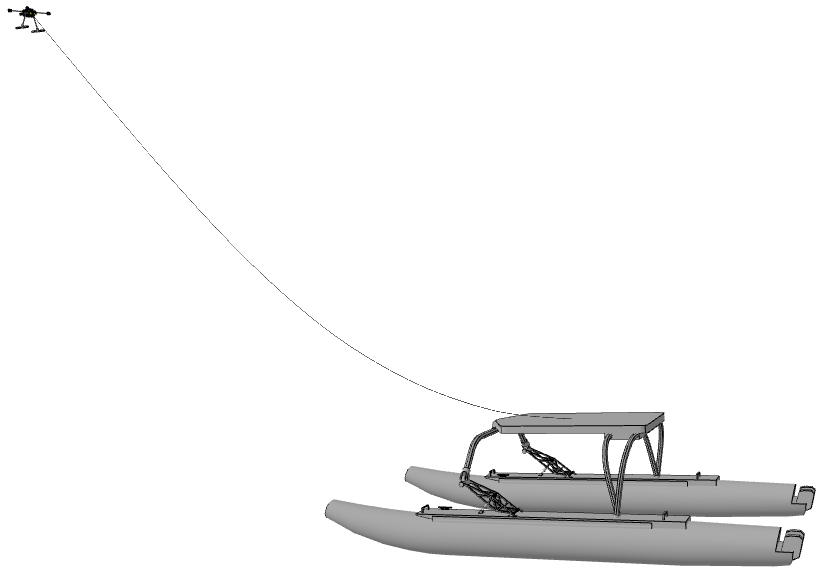
\includegraphics[height=5.5cm]{Implementation/figures/01_simulation_environment/drone_foxglove_side.png}}
        \label{fig:tether_foxglove_side}
    }
    \hfill
    \subfloat[Top view.]{
        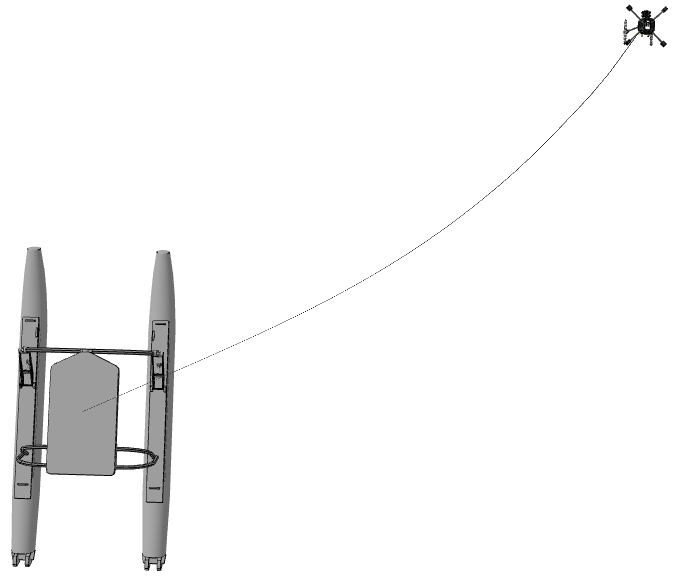
\includegraphics[height=5.5cm]{Implementation/figures/01_simulation_environment/drone_foxglove_top.png}
        \label{fig:tether_foxglove_top}
    }
    \caption{The tether between the \gls{usv} and the \gls{uav}, displayed in Foxglove.}
    \label{fig:tether_foxglove}
\end{figure}

In this type of model, the mass of the tether is concentrated at the nodes, and the segments between them have no mass, as shown in Figure~\ref{fig:tether_chain}. The motion of each free node $i$ follows from Newton's second law, with the forces shown in Figure~\ref{fig:tether_forces},
\begin{equation}
    m_i\,\ddot{\mathbf{p}}_i = \mathbf{T}_{i-1} + \mathbf{T}_i + \mathbf{F}^{\text{bend}}_i + m_i\mathbf{g} + \mathbf{F}^{\text{drag}}_i,
    \label{eq:tether_node}
\end{equation}
where $m_i$ and $\mathbf{p}_i$ are the mass and the position of the node, $\mathbf{T}_{i-1}$ and $\mathbf{T}_i$ are the tensions of the two adjacent segments, $\mathbf{F}^{\text{bend}}_i$ is the force due to the bending of the tether at the node, and $\mathbf{F}^{\text{drag}}_i$ is the drag, which opposes the velocity of the node. The magnitude of the tension of a segment depends on its elongation and on the rate at which it changes,
\begin{equation}
    T =
    \begin{cases}
        EA\,\eta + BA\,\dot{\eta}, & \eta > 0,\\
        0, & \eta \le 0,
    \end{cases}
    \qquad \eta = \frac{\ell - \ell_0}{\ell_0},
    \label{eq:tether_tension}
\end{equation}
where $\ell = \|\mathbf{p}_i - \mathbf{p}_{i-1}\|$ is the current length of the segment, the distance between its two nodes, $\ell_0$ is its unstretched length, $EA$ is the axial stiffness, and $BA$ is the damping coefficient, which is defined through the damping ratio given in Table~\ref{tab:tether_parameters}. A segment that is shorter than its unstretched length carries no tension, so the tether can go slack. The accelerations are then integrated in time to obtain the new position and velocity of every node. The end nodes are not integrated, since their motion is imposed by the vehicles, and the forces at these nodes are the forces that the tether exerts on them.

\begin{figure}[!htbp]
    \centering
    \subfloat[Tether divided into nodes and segments.]{
        \begin{tikzpicture}[
            node/.style={circle, fill=black, inner sep=1.6pt},
            note/.style={font=\scriptsize, align=center},
            ptr/.style={-{Stealth[length=4pt]}, thin, gray}
        ]
            % Node positions along a sagging cable
            \foreach \k in {0,...,6} {
                \pgfmathsetmacro{\t}{\k/6}
                \pgfmathsetmacro{\x}{5.4*\t}
                \pgfmathsetmacro{\y}{1.5*\t-1.1*4*\t*(1-\t)}
                \coordinate (n\k) at (\x,\y);
            }
            % Segments
            \foreach \k in {0,...,5} {
                \pgfmathtruncatemacro{\kk}{\k+1}
                \draw[thick] (n\k) -- (n\kk);
            }
            % Free nodes
            \foreach \k in {1,...,5} {
                \node[node] at (n\k) {};
            }
            % End points: attached to the vehicles
            \draw[fill=gray!30] ($(n0)+(-0.17,-0.17)$) rectangle ($(n0)+(0.17,0.17)$);
            \draw[fill=gray!30] ($(n6)+(-0.17,-0.17)$) rectangle ($(n6)+(0.17,0.17)$);
            \node[note] at ($(n0)+(0,-0.55)$) {Attached\\to the \gls{usv}};
            \node[note] at ($(n6)+(0,0.6)$) {Attached\\to the \gls{uav}};
            % Annotations
            \node[note] (lnode) at ($(n2)+(0,-0.95)$) {Node $i$\\(lumped mass)};
            \draw[ptr] (lnode.north) -- ($(n2)+(0,-0.1)$);
            \node[note] (lseg) at ($(n4)+(-1.2,0.95)$) {Segment\\(spring and damper)};
            \draw[ptr] (lseg.south) -- ($($(n3)!0.5!(n4)$)+(0,0.05)$);
        \end{tikzpicture}
        \label{fig:tether_chain}
    }
    \hfill
    \subfloat[Forces on a node.]{
        \begin{tikzpicture}[
            node/.style={circle, fill=black, inner sep=1.6pt},
            force/.style={-{Stealth[length=6pt]}, very thick, red!70!black},
            lab/.style={font=\scriptsize}
        ]
            \coordinate (c) at (0,0);
            \coordinate (a) at (-2.2,0.9);
            \coordinate (b) at (2.2,0.5);
            % Neighbouring segments (spring symbol)
            \draw[decorate, decoration={zigzag, segment length=5pt, amplitude=1.6pt}, gray!60] (c) -- (a);
            \draw[decorate, decoration={zigzag, segment length=5pt, amplitude=1.6pt}, gray!60] (c) -- (b);
            \node[node] at (a) {};
            \node[node] at (b) {};
            \node[node, inner sep=2.4pt] at (c) {};
            \node[lab, above=3pt] at (a) {node $i-1$};
            \node[lab, above=3pt] at (b) {node $i+1$};
            \node[lab, below right] at (c) {node $i$};
            % Forces on node i
            \draw[force] (c) -- ($(c)!1.5cm!(a)$) node[lab, midway, above, sloped, black, inner sep=2pt] {$\mathbf{T}_{i-1}$};
            \draw[force] (c) -- ($(c)!1.5cm!(b)$) node[lab, midway, above, sloped, black, inner sep=2pt] {$\mathbf{T}_{i}$};
            \draw[force] (c) -- (0,-1.1) node[lab, below, black] {$m_i\mathbf{g}$};
            % Velocity and drag
            \draw[-{Stealth[length=5pt]}, thin, gray, dashed] (c) -- (0.75,0.8) node[lab, right, black] {$\mathbf{v}_i$};
            \draw[force] (c) -- (-0.75,-0.8) node[lab, left, black] {$\mathbf{F}^{\text{drag}}_i$};
        \end{tikzpicture}
        \label{fig:tether_forces}
    }
    \caption{Lumped-mass model of the tether.}
    \label{fig:tether_model}
\end{figure}

The parameters of the model are the mass per unit length, which gives the mass $m_i$ of each node in~\eqref{eq:tether_node}, the axial stiffness $EA$ and the damping ratio, which define the tension in~\eqref{eq:tether_tension}, the bending stiffness, and the drag coefficients. Their values are given in Table~\ref{tab:tether_parameters}, together with the number of segments and the time step used to integrate the equations. The mass per unit length and the diameter are based on commercial micro-tethers for \glspl{uav} that provide power and data \cite{elistair_safet2,linden_microtethers}. The axial stiffness is lower than that of a real tether, which would require an even smaller time step for the integration to remain stable, but under the tensions of a few newtons found in this work it already stretches the tether by less than $0.1\,\%$. The length of the tether is not fixed, and it is changed by the winch described in Section~\ref{sec:tether_winch}.

\begin{table}[!htbp]
    \centering
    \caption{Parameters of the simulated tether.}
    \label{tab:tether_parameters}
    \begin{tabular}{lcc}
        \toprule
        \textbf{Parameter} & \textbf{Value} & \textbf{Unit} \\
        \midrule
        Diameter & $4$ & $\text{mm}$ \\
        Mass per unit length & $0.020$ & $\text{kg/m}$ \\
        Axial stiffness, $EA$ & $10^4$ & $\text{N}$ \\
        Damping ratio (relative to critical) & $0.8$ & -- \\
        Bending stiffness & $2\times 10^{-5}$ & $\text{N}\cdot\text{m}^2$ \\
        Transverse drag coefficient & $1.2$ & -- \\
        Axial drag coefficient & $0.005$ & -- \\
        Density of the surrounding air & $1.225$ & $\text{kg/m}^3$ \\
        Number of segments & $30$ & -- \\
        Integration time step & $0.02$ & $\text{ms}$ \\
        \bottomrule
    \end{tabular}
\end{table}

The tether is coupled to the vehicles by a \gls{ros} node, as shown in Figure~\ref{fig:tether_coupling}. At each step, the node reads the position and the velocity of the two ends of the tether, the winch on the deck of the \gls{usv} and the centre of the body of the \gls{uav}, and gives them to MoorDyn. MoorDyn imposes them as the motion of the ends of the tether, integrates the tether over the step, and returns the force vector at each end, which is applied to the vehicles in Gazebo.

\begin{figure}[!htbp]
    \centering
    % same style as the block diagrams of Figures 1.2 and 4.28
    \definecolor{simfill}{RGB}{253, 242, 228}
    \definecolor{simline}{RGB}{214, 140, 60}
    \begin{tikzpicture}[
        x=1cm, y=1cm,
        group/.style={draw=simline, fill=simfill, rounded corners=2pt, line width=0.6pt},
        block/.style={draw=simline, fill=white, rounded corners=2pt, minimum width=1.9cm, minimum height=0.8cm,
                      align=center, font=\footnotesize, line width=0.6pt},
        title/.style={font=\footnotesize\bfseries},
        flow/.style={-{Stealth[length=4pt]}, line width=0.6pt, black!75},
        list/.style={font=\scriptsize, black!80, align=left, inner sep=2pt}
    ]
        % Gazebo
        \draw[group] (0,0) rectangle (2.6,3.4);
        \node[title] at (1.3,3.05) {Gazebo};
        \node[block] at (1.3,2.0) {\gls{usv}};
        \node[block] at (1.3,0.8) {\gls{uav}};

        % MoorDyn
        \draw[draw=black!50, densely dashed, rounded corners=2pt, line width=0.6pt] (8.8,0) rectangle (11.6,3.4);
        \node[title] at (10.2,1.85) {MoorDyn};
        \node[font=\scriptsize, black!60] at (10.2,1.45) {tether dynamics};

        % Data exchange
        \draw[flow] (2.6,2.3) -- (8.8,2.3);
        \node[list, anchor=south] at (5.7,2.4) {%
            $\bullet$ Position of the tether ends\\
            $\bullet$ Velocity of the tether ends};
        \draw[flow] (8.8,1.1) -- (2.6,1.1);
        \node[list, anchor=north] at (5.7,1.0) {%
            $\bullet$ Force vector at the winch\\
            $\bullet$ Force vector at the \gls{uav}};
    \end{tikzpicture}
    \caption{Data exchange between the simulation and the tether.}
    \label{fig:tether_coupling}
\end{figure}



%%%%%%%%%%%%%%%%%%%%%%%%%%%%%%%%%%%%%%%%%%%%%%%%%%%%%%%%%%%%%%%%%%%%%%%%
\subsection{Tether Winch}
\label{sec:tether_winch}

The model of the tether used by the controllers in Section~\ref{sec:system_modeling} assumes that its slack is kept close to a constant value $\varepsilon_0$, which requires a mechanism that adjusts the length of the tether as the vehicles move. In a real system, the winch spools the tether in and out, and in simulation it is represented by a virtual winch that varies the length of the tether.

At each step, the virtual winch reads the distance $d$ between the winch and the \gls{uav} and computes the tether length $L_{\text{ref}}$ that gives the desired slack,
\begin{equation}
    L_{\text{ref}} = \frac{d}{1-\varepsilon_0},
    \label{eq:winch_length}
\end{equation}
which it then applies as the length of the tether in MoorDyn. Close to the deck, the winch can instead pull the tether with a constant force of $4\,\text{N}$, about a fifth of the weight of the \gls{uav}, raised gradually when the pull starts.
A real system cannot follow the variations of the length instantly, because of the speed of the winch and the delay in the measurement of the distance. To account for this limitation, the rate of change of the length is limited to $v_{\text{winch}} = 2\,\text{m/s}$, which makes the slack deviate from $\varepsilon_0$ when the distance changes faster than the system can follow.

To evaluate the effect of the slack ratio, the \gls{uav} flew the same $60\,\text{s}$ trajectory with $\varepsilon_0 = 2\%$, $5\%$, and $10\%$, moving along $x$ up to $10\,\text{m}$ to each side of the \gls{usv}, which held its position, so that the distance between the winch and the \gls{uav} varied between about $5$ and $14\,\text{m}$. Figure~\ref{fig:winch_shape} shows the shape of the tether for each value, and a larger slack naturally makes the tether sag more between the vehicles. Figure~\ref{fig:winch_tension} shows the tension at the \gls{uav} as a function of the distance between the winch and the \gls{uav}, averaged over intervals of $1\,\text{m}$, with the band showing its spread along the trajectory. For every slack ratio, the tension grows almost linearly with the distance, since the weight of the tether that the \gls{uav} supports increases with it. A larger slack lowers the whole curve, since a tether that sags more needs less tension to hold its own weight. Table~\ref{tab:winch_slack} quantifies these results. From $\varepsilon_0 = 2\%$ to $10\%$, the mean tension decreases by $22\%$ and the maximum by $15\%$.

\begin{figure}[!b]
    \centering
    \subfloat[$\varepsilon_0 = 2\%$.]{
        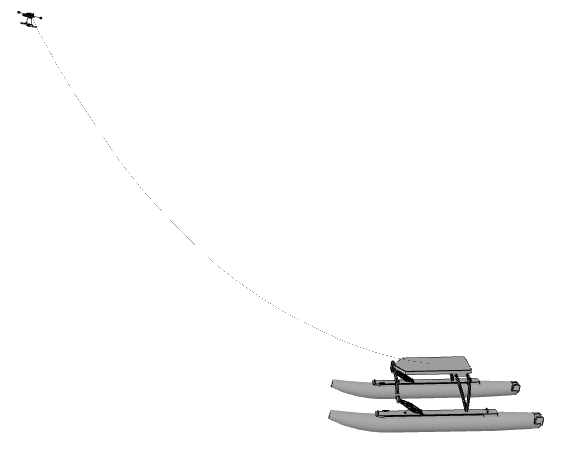
\includegraphics[width=0.32\textwidth]{Implementation/figures/01_simulation_environment/slack_2.png}
        \label{fig:winch_shape_2}
    }
    \hfill
    \subfloat[$\varepsilon_0 = 5\%$.]{
        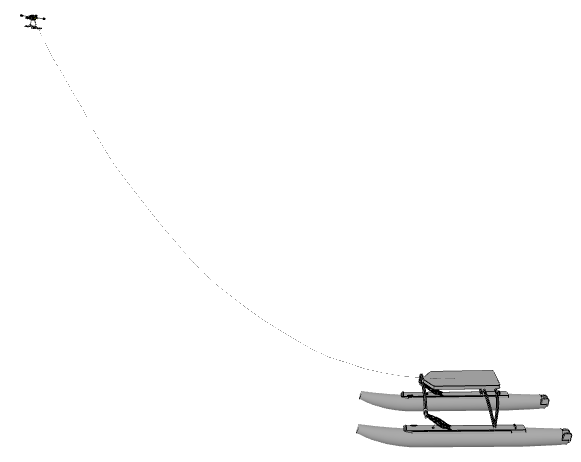
\includegraphics[width=0.32\textwidth]{Implementation/figures/01_simulation_environment/slack_5.png}
        \label{fig:winch_shape_5}
    }
    \hfill
    \subfloat[$\varepsilon_0 = 10\%$.]{
        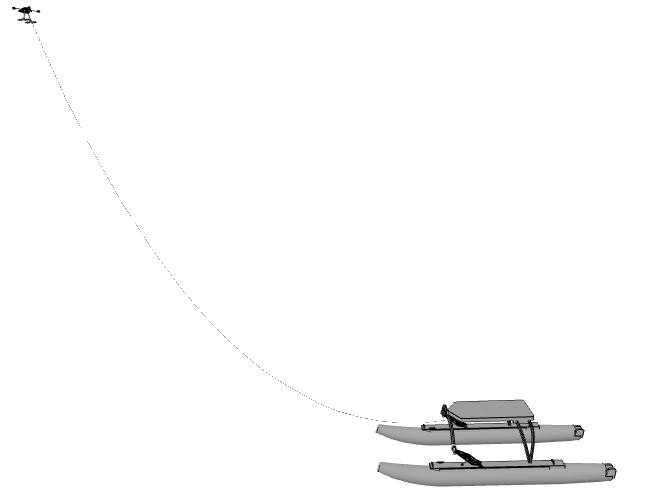
\includegraphics[width=0.32\textwidth]{Implementation/figures/01_simulation_environment/slack_10.png}
        \label{fig:winch_shape_10}
    }
    \caption{Shape of the tether for different slack ratios.}
    \label{fig:winch_shape}
\end{figure}

\begin{figure}[!htbp]
    \centering
    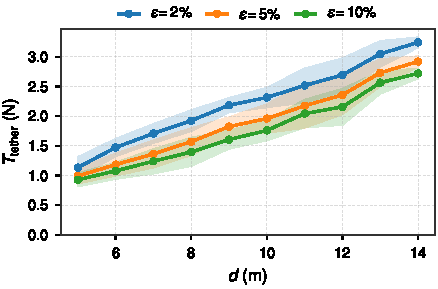
\includegraphics{Implementation/figures/01_simulation_environment/slack_tension_distance.pdf}
    \caption{Tension at the \gls{uav} as a function of the distance, for different slack ratios.}
    \label{fig:winch_tension}
\end{figure}

\begin{table}[!htbp]
    \centering
    \caption{Tension at the \gls{uav} for different slack ratios.}
    \label{tab:winch_slack}
    \begin{tabular}{ccc}
        \toprule
        \textbf{$\varepsilon_0$} & \textbf{Mean} (N) & \textbf{Maximum} (N) \\
        \midrule
        $2\%$  & $2.07$ & $3.38$ \\
        $5\%$  & $1.78$ & $3.08$ \\
        $10\%$ & $1.62$ & $2.88$ \\
        \bottomrule
    \end{tabular}
\end{table}

These tensions are small compared with the weight of the \gls{uav}, which is $20.2\,\text{N}$, so the tension alone does not determine the choice of $\varepsilon_0$. The choice is instead a compromise on the amount of slack. Some slack is needed to absorb disturbances and avoid sudden tension spikes at the \gls{uav}, but too much makes the tether harder to manage and more likely to tangle. A value of $\varepsilon_0 = 5\%$ is used in the remainder of this work.